\documentclass[twocolumn]{article}
\usepackage[utf8]{inputenc}

\usepackage[english]{babel}
\usepackage[dvinames]{xcolor}
%\usepackage[compact,small]{titlesec}
\usepackage{booktabs}
\usepackage{multirow}
\usepackage{amsfonts,amsmath,amssymb}
\usepackage{marginnote}
\usepackage[top=1.8cm, bottom=1.8cm, outer=1.8cm, inner=1.8cm, heightrounded, marginparwidth=2.5cm, marginparsep=0.5cm]{geometry}
\usepackage{enumitem}
%\setlist{noitemsep,parsep=2pt}
%\newcommand{\highlight}[1]{\textcolor{kuleuven}{#1}}
\usepackage{pythonhighlight}
\usepackage{hyperref}
\usepackage{cleveref}
\usepackage{graphicx}
\usepackage{mathtools}
\usepackage{tikz}
\usepackage{caption}
\usepackage{subcaption}
\usepackage{float}

\title{Topological Data Analysis 2023/24 \\ Project: Sensors}
\author{Noah Novšak and Tim Kalan}
\date{january 2023}

\begin{document}

\maketitle

\section{Introduction}
The problem of sensor coverage is usually presented as satellites orbiting Earth and providing a signal to the population. One possible question is how to distribute these satellites so Earth's surface is completely covered. A variation asks what radius each satellite needs to cover so that a given distribution covers everything. Additionally, we can ask how far each satellite must broadcast so that all of the satellites can communicate with each other.

In this project, we look at a simplified version of this problem, given several points on the unit sphere. The sensors gather data and form a network with parameters $r$ and $R$.
\begin{itemize}
    \item Each sensor gathers data from the surrounding area in a circle of radius $R$.
    \item Each sensor can communicate with other sensors at most $r$ away.
\end{itemize}

\subsection{Project goal}  
Determine $r$ and $R$, so that
\begin{enumerate}
    \item the numbers $r$ and $R$ are as small as possible (that would decrease the cost of sensors),
    \item the sensor network is connected (i.e., the Vietoris-Rips graph is connected),
    \item the sensor network covers the whole sphere (the Čech complex should be homotopy equivalent to the sphere, i.e., the Euler characteristic of the Čech complex should be that of a sphere).
\end{enumerate}

Furthermore, once the parameters $r$ and $R$ are established, the program should return a list of obsolete sensors, i.e., sensors whose removal would not change the desired properties 2. and 3. of the sensor network.

\subsection{The data}
We were given a set of $54$ points on a sphere for which the radii had to be found. Plotting the dataset \ref{fig:data} shows that the points are reasonably uniformly spread out on the sphere.

\begin{figure}[H]
    \centering
    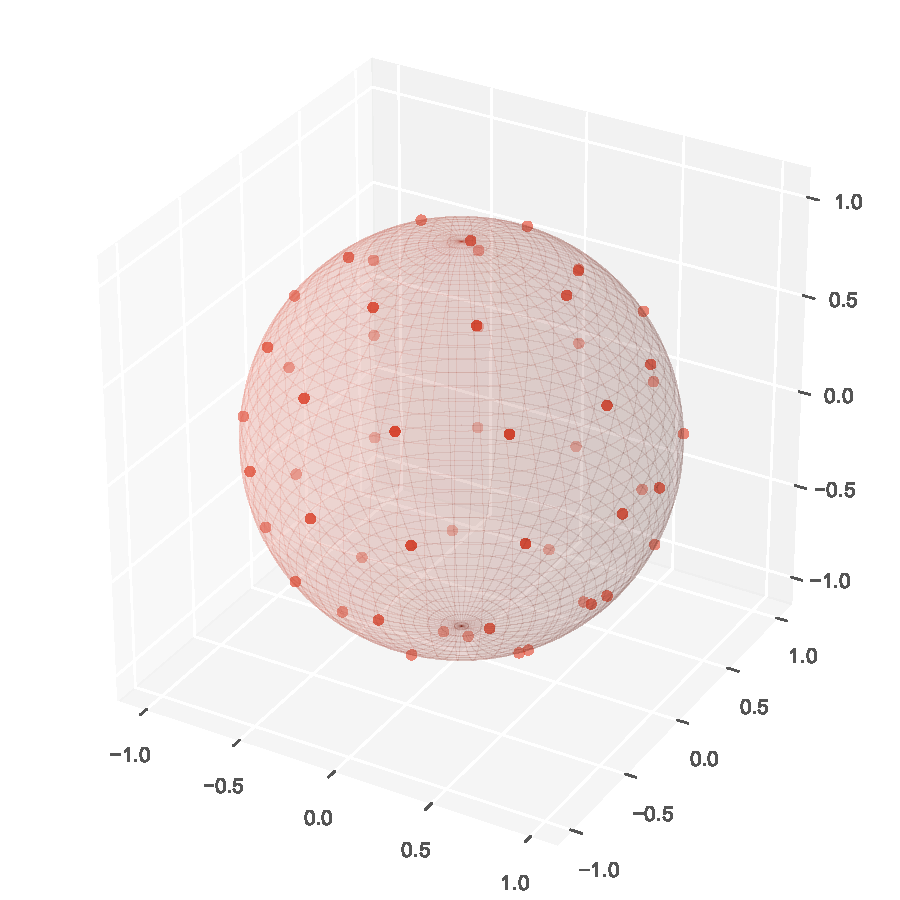
\includegraphics[width=\columnwidth]{fig/data}
    \caption{Given points on the unit sphere representing sensor locations around Earth.}
    \label{fig:data}
\end{figure}

\section{Methods}
The project is split into four parts. The following section describes the methods used in each of them. 

\subsection{Coverage radius \textit{R}}

\subsubsection{Čech complex}
As the instructions suggest, one of the ways to find the minimal coverage radius is to construct a Čech complex out of the given points and increase the radius until it is homotopy equivalent to a sphere. We found no (Python) libraries for computing this, so we implemented our generator using only a library for the MiniBall algorithm. The generator is very inefficient, as it goes through all possible subsets of the points of a given size. For each subgroup, it checks (via the MiniBall algorithm) whether it is a simplex in the Čech complex of the given radius. With this, we generated the $2$-skeleton of the complex, which should be enough for our purposes. 

Then, the idea was to check the connectivity of such a complex and its Euler characteristic. Connectivity was computed via a depth-first search on the $1$-skeleton of the complex. If only one component was found, the complex was deemed connected. The Euler characteristic was then computed in the standard way by counting simplices of different dimensions and adding/subtracting them.

With these two characteristics of the complex, we could run a bisection to get the minimal radius at which the complex was connected and had the Euler characteristic of a sphere.

\subsubsection{Alpha complex}
The Alpha complex is topologically equivalent to the Čech complex but is much easier to compute, especially considering that it is part of the \texttt{gudhi} library. We decided to double-check our results by also considering this complex.

The general idea and method were the same: generate the complex for a given radius and check whether it is connected and has the correct Euler characteristic. With this procedure in place, we can again run a bisection like with the Čech complex to obtain the result.

\begin{figure}[H]
    \centering
    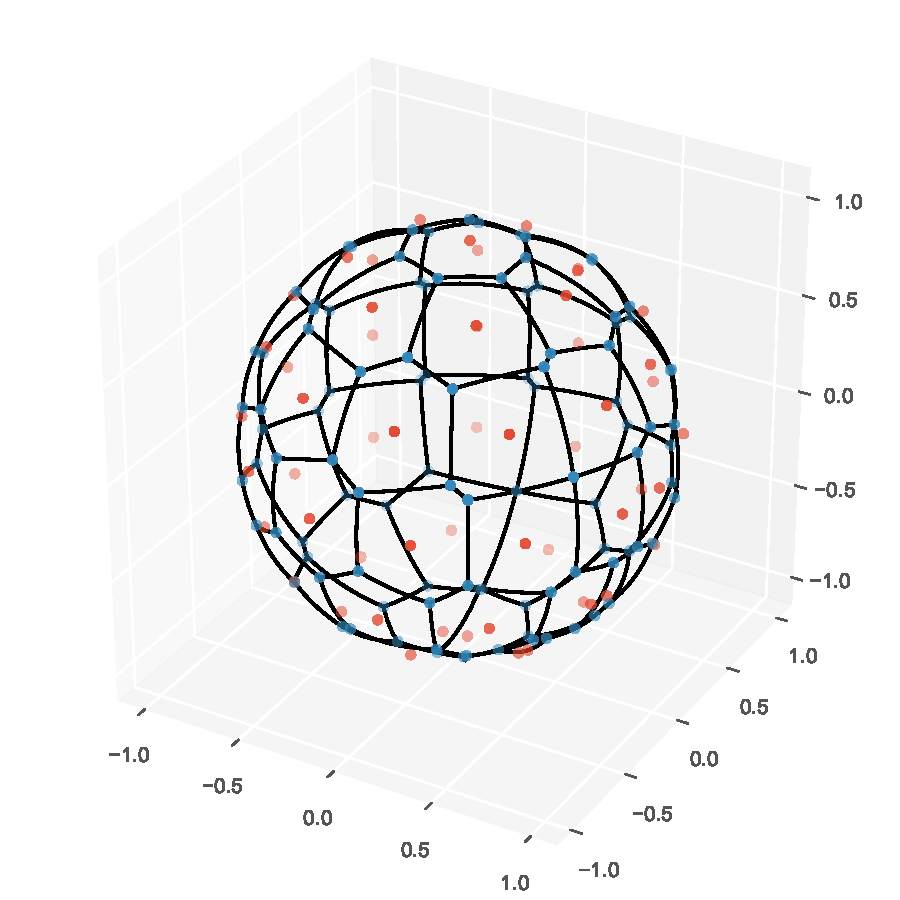
\includegraphics[width=\columnwidth]{fig/voronoi}
    \caption{Sensor locations (red) and vertices of the spherical Voronoi diagram (blue), representing the potentially furthest points from the sensors.}
    \label{fig:voronoi}
\end{figure}

\subsubsection{Spherical Voronoi diagram}
An alternative way to quickly compute the coverage radius was to compute the spherical Voronoi diagram instead. Of course, we can only do this because we are dealing with points on a sphere, but given that fact, we can use the \texttt{scipy.spatial} library to compute $R$ much more efficiently. The Voronoi diagram~\ref{fig:voronoi} will give us the points that are furthest away from each local triplet, so taking the maximal distance to any of those points, we get our coverage radius $R$.

\subsection{Communication radius \textit{r}}
Here, we considered two methods, but they are pretty similar. As the instructions suggested, we looked at the Vietoris-Rips complex generated by the dataset.

\subsubsection{Persistent homology}
The first approach was via persistent homology. We used the \texttt{ripser} library to generate the persistence diagram of the Vietoris-Rips complex on the given points. As we are interested in the connectivity of the complex, we only need to look at $H_0$ to find our answer.

\begin{figure}[H]
    \centering
    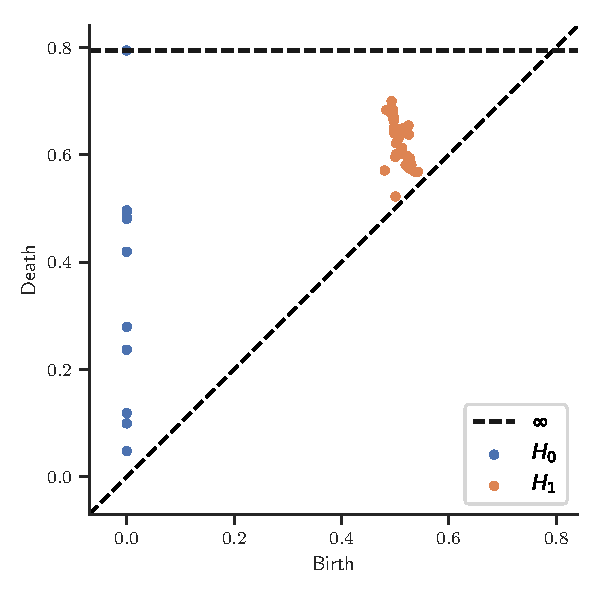
\includegraphics[width=\columnwidth]{fig/persistence}
    \caption{Persistance diagram showing the last $H_0$ dies at $r = 0.49$, meaning all the sensors are now connected. Interestingly, many $H_1$ groups begin to appear around the same time and die shortly after.}
    \label{fig:persistance}
\end{figure}

\subsubsection{Vietoris-Rips and bisection}
In the alternative approach, we also use the Vietoris-Rips complex. But this time, instead of computing the entire persistence diagram, we generate the complex only for a select number of radii using the \texttt{gudhi} library. Our idea was to find the radius by bisecting the interval $[0, 1]$ and checking when the complex is connected. 

To check whether the complex is connected, we looked at the complex's one-dimensional skeleton as a graph and ran a depth-first search from an arbitrary vertex. If all other vertices were visited, the graph is connected; thus, the complex is also.

\subsection{Obsolete points}
We can now find potentially obsolete points after calculating the minimal communication and coverage radii using the methods above. Our first idea was to look at the simplices in the Čech complex of dimension $3$ or higher and take those points as candidates for obsolete points. However, we only had $50$ points in our dataset and wanted the method to work without computing the Čech complex (e.g. when using Voronoi diagrams), so we opted for a more straightforward strategy. First, loop over the points and recalculate the radii, ignoring a single point. Each point is deemed obsolete if the radii obtained are smaller/similar to the original. This was checked by first recomputing the radii and then checking for similarity with \texttt{numpy.allclose}.

Further, the idea was to look at the combinations of these points, but as only one obsolete point was found, no combinations needed to be considered. The project code still includes this functionality (unused in this case).

\begin{figure}[H]
    \centering
    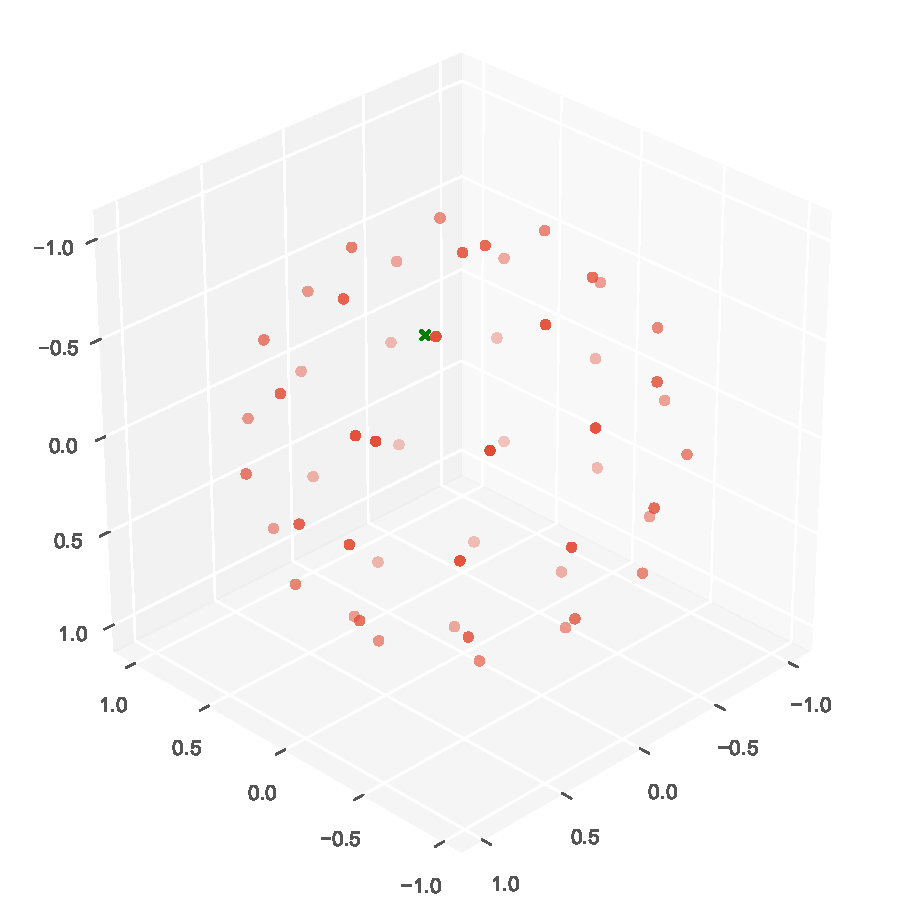
\includegraphics[width=\columnwidth]{fig/obsolete}
    \caption{The initial dataset has one obsolete point (green \texttt{X}).}
    \label{fig:obsolete}
\end{figure}

\subsection{Data generator}
The first idea for data generation was to use a Fibonacci lattice. This relatively simple method generates points on the sphere by mapping the Fibonacci spiral onto a sphere. The resulting points are relatively evenly distributed but definitely not optimal. However, the lattice is still a good starting point for further optimization. Using our methods for computing the coverage radius $R$ (optimizing for $r$ is trivial), we can find an optimal placement of points with any number of existing optimization techniques (in this case, we used \texttt{scipy.optimize.minimize}).
If it is too slow, an alternative to computing $R$ is implementing a repelling force (i.e., Colomb's law) between the sensors and effectively transforming the question into the Thomson problem.

\begin{figure}[H]
    \centering
    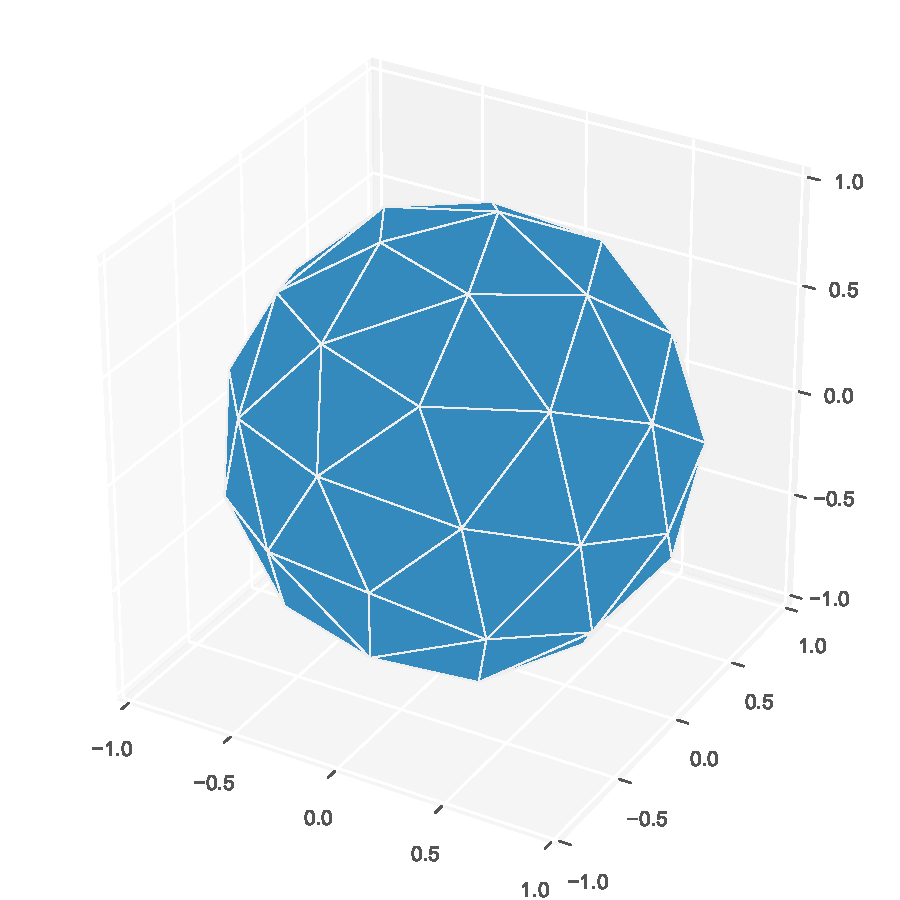
\includegraphics[width=\columnwidth]{fig/optimised}
    \caption{Optimized placement of $50$ sensors with parameters $R = 0.3238$, and $r = 0.545$.}
    \label{fig:optimised}
\end{figure}

\begin{figure}[H]
    \centering
    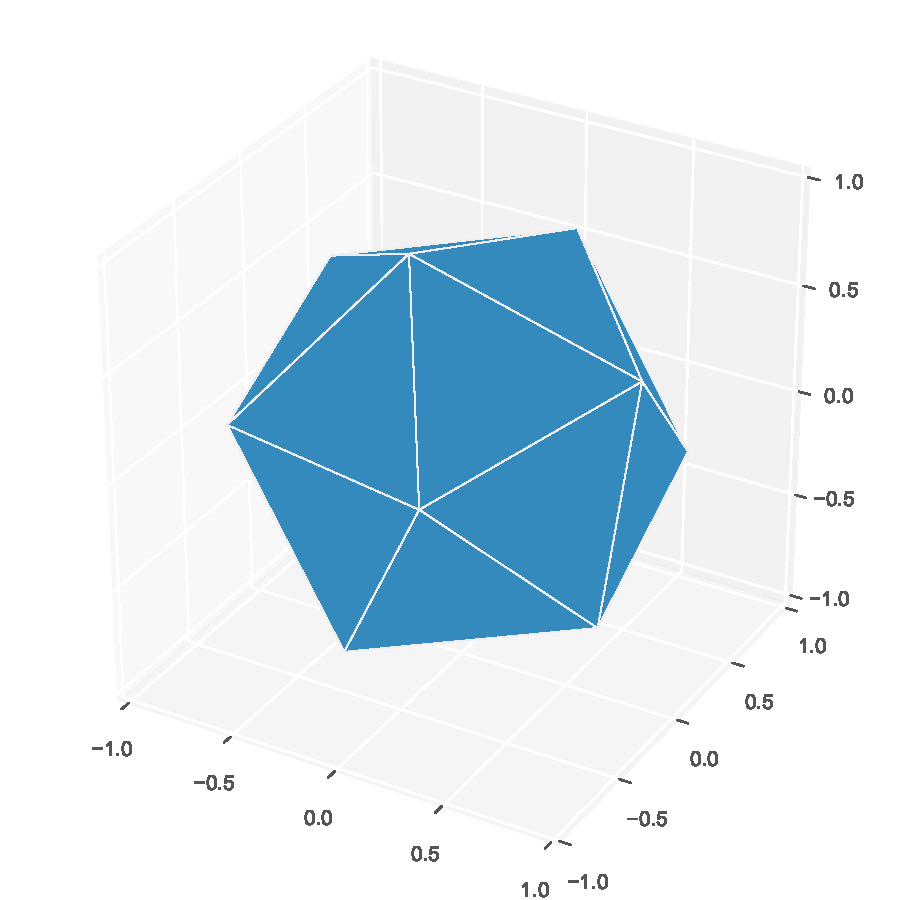
\includegraphics[width=\columnwidth]{fig/icosahedron}
    \caption{The optimization only has stable solutions for specific numbers of vertices. One such example is the icosahedron for $12$ vertices.}
    \label{fig:icosahedron}
\end{figure}

\section{Results}
This section contains a summary of results obtained with all of the methods.

\subsection{Coverage radius \textit{R}}
\begin{table}[h]
    \centering
    \begin{tabular}{c|c}
        Method & Value  \\
        \hline
         Čech complex & 0.3351 \\
         Alpha complex & 0.3561 \\
         Spherical Voronoi diagram & 0.3621 \\
    \end{tabular}
    \caption{There are some differences between the results stemming from the difference in measuring distances between points on a plane and a sphere.}
    \label{tab:R}
\end{table}

\subsection{Communication radius \textit{r}}
\begin{table}[h]
    \centering
    \begin{tabular}{c|c}
        Method & Value  \\
        \hline
         Vietoris-Rips persistent homology & 0.4965 \\
         Vietoris-Rips bisection & 0.4965 \\
    \end{tabular}
    \caption{In this case, both methods returned the same result.}
    \label{tab:r}
\end{table}

\subsection{Obsolete points}
Only one obsolete point was found. It lies at coordinates $(0.4994, -0.2634, -0.8253)$ and has a twin right next to it. Interestingly, its twin cannot be removed, nor can any other point with a twin be removed. We would need to allow a change in parameters on the second decimal to remove any of them. In that case, several pairs can be removed (but not simultaneously).

\subsection{Data generator}
Since the optimal communication radius $r$ is $0$ (all points in one), it only makes sense to look at $R$. Table \ref{tab:generator} shows the lowest $R$ obtained via Fibonacci lattice and point optimization.

\begin{table}[h]
    \centering
    \begin{tabular}{c|c}
        Method & Value  \\
        \hline
         Fibonacci lattice & 0.3835 \\
         Optimization & 0.3274 \\
    \end{tabular}
    \caption{Lowest coverage radius obtained.}
    \label{tab:generator}
\end{table}

\begin{thebibliography}{1}
    \bibitem{scipy}Virtanen, P., Gommers, R., Oliphant, T., Haberland, M., Reddy, T., Cournapeau, D., Burovski, E., Peterson, P., Weckesser, W., Bright, J., Van der Walt, S., Brett, M., Wilson, J., Millman, K., Mayorov, N., Nelson, A., Jones, E., Kern, R., Larson, E., Carey, C., Polat, İ., Feng, Y., Moore, E., VanderPlas, J., Laxalde, D., Perktold, J., Cimrman, R., Henriksen, I., Quintero, E., Harris, C., Archibald, A., Ribeiro, A., Pedregosa, F., Van Mulbregt, P. \& SciPy 1.0 Contributors SciPy 1.0: Fundamental Algorithms for Scientific Computing in Python. {\em Nature Methods}. \textbf{17} pp. 261-272 (2020)

    \bibitem{Bauer2021Ripser}Bauer, U. Ripser: efficient computation of Vietoris-Rips persistence barcodes. {\em J. Appl. Comput. Topol.}. \textbf{5}, 391-423 (2021), \url{https://doi.org/10.1007/s41468-021-00071-5}

    \bibitem{gudhi} GUDHI Python modules documentation, \url{https://gudhi.inria.fr/python/latest/}

\end{thebibliography}

\end{document}